\documentclass[12pt,a4paper]{article}

% Packages
\usepackage[margin=2.5cm]{geometry}
\usepackage[utf8]{inputenc}
\usepackage[T1]{fontenc}
\usepackage{lmodern}
\usepackage{setspace}
\usepackage{amsmath,amssymb}
\usepackage{graphicx}
\usepackage{booktabs}
\usepackage{longtable}
\usepackage{float}
\usepackage{caption}
\usepackage{enumitem}
\usepackage{xcolor}
\usepackage{algorithm}
\usepackage{algpseudocode}
\usepackage[colorlinks=true,linkcolor=blue!60!black,citecolor=blue!60!black,urlcolor=blue!60!black]{hyperref}
\usepackage{titlesec}
\usepackage{fancyhdr}

\onehalfspacing

\pagestyle{fancy}
\fancyhf{}
\fancyhead[L]{\small Collignon -- Pesticide Disaggregation}
\fancyhead[R]{\small\thepage}
\renewcommand{\headrulewidth}{0.4pt}

\title{\textbf{Matching company-level pesticide reports to agricultural fields using administrative identifiers: A 14-year coverage analysis with Danish government data}}
\author{Martin Collignon\textsuperscript{1}\\[6pt]
\textsuperscript{1}Landbruget.dk, Denmark}
\date{}

\begin{document}

\maketitle
\thispagestyle{fancy}

\begin{abstract}
Pesticide application data in the European Union is typically reported at company or regional level, limiting field-level environmental risk assessment. We present a method that matches company-level spray journal records to individual georeferenced agricultural fields by exploiting a shared administrative identifier (the Danish CVR company number) and crop code, with proportional dose allocation within a configurable area tolerance (default $\pm2\%$). Validated across 14 years of Danish government data (2010--2023), the method achieves 92.7\% matching coverage in 2020, sustaining $\geq90\%$ from 2018 onward. Matching coverage measures the fraction of records successfully linked to georeferenced fields---not allocation accuracy: only 19.6\% of matched records receive unambiguous single-field allocations, while 80.4\% are distributed proportionally across multiple fields. Tolerance sensitivity analysis reveals that relaxing tolerance from 0\% to 0.5\% produces the largest coverage gain (37--48\% to 72--87\%), identifying area rounding in spray journal reporting as the dominant mismatch source. The method requires no machine learning and produces auditable allocations, but the proportional dose distribution step relies on an unvalidated uniform-intensity assumption. All input data are Danish government administrative records; spray journal data was obtained through freedom of information requests and all other sources are publicly available.

\medskip
\noindent\textbf{Keywords:} pesticide disaggregation, spatial resolution, area matching, Danish agriculture, field-level analysis, spray journal, administrative data linkage
\end{abstract}

\clearpage

%----------------------------------------------------------------------
\section{Introduction}

\subsection{The spatial resolution gap}

Spatially resolved pesticide use data is a prerequisite for environmental and health risk assessment. Across the EU, such data has historically been available only as national sales totals under Regulation (EC) No~1185/2009, which mandates farm-level use surveys only every five years at national or regional aggregation \cite{eurostat2023}. The Statistics on Agricultural Input and Output (SAIO) Regulation (EU)~2022/2379 mandates electronic recording of pesticide use from 1~January~2026, with first data transmission to Eurostat by end of 2028. However, even under SAIO, field-level spatial data is not required; Member States will collect data at the farm or holding level \cite{ec2022}. The European Commission's Farm to Fork Strategy target of 50\% reduction in pesticide use by 2030 \cite{ec2020} further underscores the need for spatially resolved monitoring data to track progress at meaningful scales.

This gap has been widely documented. Piera et al.\ \cite{piera2023} noted that absent georeferenced use data severely constrains environmental fate modelling. Balcaen et al.\ \cite{balcaen2025} observed that even advanced EU-wide mapping efforts rely on statistical downscaling rather than direct observation. The JRC has consistently identified spatial disaggregation as a key methodological challenge \cite{jrc2019}.

\subsection{Existing approaches}

The literature on spatially resolving pesticide data spans three broad categories, each sharing a fundamental limitation.

\paragraph{Sales-based and statistical downscaling.} France's NODU indicator distributes postal-code-level sales to municipalities using crop area proportions \cite{deguine2023}. Zucchini et al.\ \cite{zucchini2022} mapped 388 active substances across 9.5~million parcels in Wallonia by combining postal-code sales with crop-specific application rates from a 4\% farm survey. At broader scales, Maggi et al.\ \cite{maggi2019} produced global gridded maps (PEST-CHEMGRIDS) at $\sim$10~km resolution, and Balcaen et al.\ \cite{balcaen2025} achieved 250~m EU-wide maps by fusing PEST-CHEMGRIDS with Sentinel-derived crop type maps. These approaches lack farm identity: the same crop area in different companies receives identical estimated doses regardless of actual practices.

\paragraph{Exposure mapping and risk models.} Deguine et al.\ \cite{deguine2025} combined France's RPG parcel registry with population density for residential exposure mapping. Zucchini et al.\ \cite{zucchini2024} quantified residential pesticide exposure in Wallonia using buffer-based models. Process-based models such as SYNOPS \cite{gutsche1997,strassemeyer2017} assess risk at the field level but require the very field-level use data that is typically unavailable. California's Pesticide Use Reporting (PUR) program, operational since 1990, requires reporting at $\sim$2.6~km$^2$ sections \cite{cadpr2024}, but specific fields within sections are not identified, requiring statistical downscaling \cite{larsen2017,nuckols2007}.

\paragraph{Farm-level monitoring.} M\"ohring et al.\ \cite{moehring2020} demonstrated farm-level pesticide use quantification in Switzerland using central registry linkage, though without the field-level spatial disaggregation component presented here. EFSA has published technical reports on harmonizing pesticide use monitoring across Member States, consistently identifying the lack of georeferenced field-level data as a barrier \cite{efsa2023}.

None of these approaches exploit direct farm-identity linkage between application records and georeferenced field boundaries. The fundamental bottleneck is the absence of a shared identifier connecting ``who applied what'' to ``where their fields are.''

\subsection{Contribution}

Denmark possesses two government datasets that, combined, provide the direct linkage that existing methods lack. The Spr\o jtejournal (SJI) system requires all professional users managing more than 10~hectares to report pesticide applications annually, identifying each company by CVR number and crop code \cite{mst2024}. The FVM Marker dataset provides georeferenced field boundaries using the same CVR and crop code classification \cite{lbst2024}.

This paper makes three contributions: (1)~a data integration methodology that matches company-level pesticide records to individual fields using shared administrative identifiers, with proportional dose allocation and per-record quality scores; (2)~empirical characterization across 14~years (2010--2023), demonstrating matching coverage exceeding 90\% from 2018 onward; and (3)~tolerance sensitivity analysis identifying area rounding as the dominant mismatch source. The pipeline is open-source, underlying the landbruget.dk transparency platform.

%----------------------------------------------------------------------
\section{Data Sources}

\subsection{Spray journal data (SJI)}

The SJI system is maintained by Milj\o styrelsen under the Danish Pesticide Action Plan. SJI data is not open data; access was obtained through freedom of information requests (\textit{aktindsigt}) under the Danish Environmental Information Act. Each record contains: CVR number, F\ae llesskema (Common Application) crop code, total application area (hectares) for that crop, pesticide product name and registration number, and dosage quantity with unit. The reporting period follows the agricultural year (August~1 to July~31). The dataset contains 310,000--440,000 records per year (2010--2023). Areas are reported at company-plus-crop granularity, not per individual field, and appear to be rounded (confirmed by tolerance sensitivity analysis in Section~\ref{sec:tolerance}). SJI-reported consumption is consistently lower than independently measured sales totals \cite{mst2023}, particularly for glyphosate; disaggregated outputs therefore represent a lower bound on actual application.

\subsection{Field boundary data (FVM Marker)}

Published by Landbrugsstyrelsen via WFS at geodata.fvm.dk, FVM Marker contains 600,000--740,000 georeferenced field records per year. Each record includes: field identifier, CVR number, F\ae llesskema crop code, field area (hectares), organic farming indicator, and polygon geometry in EPSG:25832. The crop code system has been stable across the study period, with no wholesale reclassification.

\subsection{Supporting datasets}

The BMD pesticide product registry (bmd.mst.dk) provides product attributes including the Pesticide Load Indicator \cite{kudsk2018} and PFAS flags, enabling post-hoc dose-rate plausibility checks via the shared registration number. The BBR building registry and GEUS VP4 groundwater monitoring dataset support downstream proximity and contamination analyses.

\begin{table}[H]
\centering
\caption{Data sources.}
\label{tab:datasources}
\footnotesize
\begin{tabular}{@{}lllll@{}}
\toprule
Source & Authority & Period & Resolution & Access \\
\midrule
SJI & Milj\o styrelsen & 2010--2023 & Company + crop & FOI \\
FVM Marker & Landbrugsstyrelsen & 2011--2024 & Field & geodata.fvm.dk \\
BMD & Milj\o styrelsen & Cont.\ updated & Product & bmd.mst.dk \\
BBR & SDFI & Cont.\ updated & Building & bbr.dk \\
GEUS VP4 & GEUS & 1981--2025 & Borehole & DOI: 10.22008 \\
\bottomrule
\end{tabular}
\end{table}

%----------------------------------------------------------------------
\section{Methods}

\subsection{Problem formalization}

Let $R = \{r_1, \ldots, r_n\}$ denote SJI records, where each $r_i = (\text{cvr}_i, \text{crop}_i, \text{area}_i^{\text{SJI}}, \text{dose}_i)$. Let $F = \{f_1, \ldots, f_m\}$ denote FVM fields, where each $f_j = (\text{cvr}_j, \text{crop}_j, \text{area}_j^{\text{FVM}}, \text{geometry}_j)$. The disaggregation task assigns each $r_i$ to fields $M_i \subseteq F$ satisfying:

\medskip
\noindent\textbf{Identity constraint:}
\begin{equation}
\text{cvr}_j = \text{cvr}_i \;\wedge\; \text{crop}_j = \text{crop}_i \quad \forall\, j \in M_i
\end{equation}

\noindent\textbf{Area matching:}
\begin{equation}
\frac{|\text{area}_i^{\text{SJI}} - \sum_{j \in M_i} \text{area}_j^{\text{FVM}}|}{\text{area}_i^{\text{SJI}}} \leq \tau, \quad \text{with default } \tau = 0.02 \; (2\%)
\end{equation}

\noindent\textbf{Proportional allocation:}
\begin{equation}
\text{dose\_field}_j = \text{dose}_i \times \frac{\text{area}_j^{\text{FVM}}}{\sum_{k \in M_i} \text{area}_k^{\text{FVM}}}
\end{equation}
preserving mass balance.

\noindent\textbf{Area-match quality score:}
\[
\text{score} = \max\!\big(0,\; 1 - |\Delta\text{area}\%| \,/\, \tau\big)
\]
This linear function measures area-match precision only; it does not reflect allocation reliability, which depends on the number of fields in the matched set. In 2021, the median score across 1,671,454 disaggregated records is 0.98 (mean 0.93), with 27.1\% receiving the maximum score of 1.0.

\subsection{Matching algorithm}

The algorithm processes unmatched records through three strategies in strict sequential order. Each strategy operates only on records not yet matched by preceding strategies.

\begin{algorithm}[H]
\caption{Pesticide disaggregation via sequential area matching.}
\label{alg:disagg}
\begin{algorithmic}[1]
\Require $R$ (SJI records), $F$ (FVM fields), $\tau$ (tolerance, default 0.02)
\Ensure $D$ (disaggregated field-level records)
\State $\textit{pending} \gets R$;\quad $D \gets \emptyset$
\Statex
\Comment{\textbf{Strategy~1: Full area match (all fields)}}
\For{each $r$ in \textit{pending}}
    \State $F_{\text{match}} \gets \{f \in F : f.\text{cvr} = r.\text{cvr} \;\wedge\; f.\text{crop} = r.\text{crop}\}$
    \State $A_{\text{total}} \gets \sum_{f \in F_{\text{match}}} f.\text{area}$
    \If{$A_{\text{total}} > 0$ \textbf{and} $|r.\text{area} - A_{\text{total}}| / r.\text{area} \leq \tau$}
        \State allocate $r$ proportionally across $F_{\text{match}}$
        \State remove $r$ from \textit{pending}
    \EndIf
\EndFor
\Statex
\Comment{\textbf{Strategy~2: Non-organic fallback}}
\For{each $r$ in \textit{pending}}
    \State $F_{\text{match}} \gets \{f \in F : f.\text{cvr} = r.\text{cvr} \;\wedge\; f.\text{crop} = r.\text{crop} \;\wedge\; \lnot f.\text{organic}\}$
    \State (same area-match test and allocation as S1)
\EndFor
\Statex
\Comment{\textbf{Strategy~3: Partial field coverage}}
\For{each $r$ in \textit{pending}}
    \State $F_{\text{match}} \gets \{f \in F : f.\text{cvr} = r.\text{cvr} \;\wedge\; f.\text{crop} = r.\text{crop}\}$
    \If{$|F_{\text{match}}| = 1$ \textbf{and} $r.\text{area} < F_{\text{match}}[0].\text{area}$}
        \State assign entire dose to the single field
        \State flag as partial coverage (quality score $= 0.8$)
    \EndIf
\EndFor
\end{algorithmic}
\end{algorithm}

\textbf{Strategy~1 (S1)} retrieves all FVM fields sharing the same CVR and crop code, and tests whether their total area matches the reported application area within tolerance. When matched, dosage is distributed proportionally by field area. S1 handles $\sim$92\% of records for recent years.

\textbf{Strategy~2 (S2)} re-evaluates unmatched records after excluding organic fields, addressing companies operating both organic and conventional fields for the same crop. S2 contributes 0--0.2 additional percentage points at 2\% tolerance, declining to zero by 2023.

\textbf{Strategy~3 (S3)} handles cases where a single registered field exists for a CVR+crop combination and the reported area is less than the field area, representing partial-field treatment.

\subsection{Temporal alignment}

SJI year~$X$ is matched against FVM field boundaries from year~$X+1$. The F\ae llesskema submitted in spring of year~$X+1$ declares field boundaries and crops for the \textit{preceding} agricultural year. Under Y+0 alignment (matching SJI year~$X$ against FVM year~$X$), the FVM dataset instead describes the growing season \textit{before} the one in which the pesticides were applied. Because Danish farms practice crop rotation, Y+0 alignment produces systematic crop code mismatches.

Table~\ref{tab:alignment} quantifies this effect. With Y+0 alignment, coverage at 2\% tolerance drops from 82--93\% to 6--9\% across all tested years---an 82--84 percentage point reduction that is consistent and stable. The near-total failure of Y+0 matching confirms that the temporal offset is not a calibration choice but a structural requirement of the Danish administrative reporting cycle.

\begin{table}[H]
\centering
\caption{Y+1 versus Y+0 matching coverage (S1) at 2\% area tolerance.}
\label{tab:alignment}
\begin{tabular}{@{}lccc@{}}
\toprule
SJI Year & Y+1 coverage & Y+0 coverage & Difference \\
\midrule
2018 & 90.4\% & 8.2\% & +82.2\,pp \\
2019 & 91.5\% & 9.4\% & +82.1\,pp \\
2020 & 92.6\% & 9.3\% & +83.3\,pp \\
2021 & 91.9\% & 9.3\% & +82.6\,pp \\
2022 & 91.2\% & 6.8\% & +84.4\,pp \\
2023 & 90.0\% & 6.3\% & +83.7\,pp \\
\bottomrule
\end{tabular}
\end{table}

\noindent\textit{Note: SJI~2015 is excluded because FVM~2015 (Y+0 target) contains NULL CVR values (the 2014 anomaly). The 6--9\% Y+0 coverage represents farmers who happen to grow the same crop on the same total area in consecutive years.}

\subsection{Implementation}

The pipeline is implemented in Python using DuckDB with spatial extensions for in-process SQL-based data processing. Data flows through bronze (raw), silver (cleaned), and gold (analysis-ready) layers. The complete source code and a validation script reproducing all reported results are open-source.

%----------------------------------------------------------------------
\section{Results}

\subsection{Longitudinal coverage (2010--2023)}

Table~\ref{tab:coverage} presents coverage across 14~years at the default 2\% tolerance.

\begin{table}[H]
\centering
\caption{Disaggregation coverage by year at 2\% area tolerance.}
\label{tab:coverage}
\begin{tabular}{@{}lrrrr@{}}
\toprule
Year & SJI Records & S1 matched & S2 additional & Coverage \\
\midrule
2010 & 390,956 & 217,819 & 0 & 55.7\% \\
2011 & 407,352 & 256,043 & 994 & 63.1\% \\
2012 & 404,289 & 252,161 & 909 & 62.6\% \\
2013 & 422,795 & 280,606 & 800 & 66.6\% \\
2014 & 440,059 & 0 & 0 & 0.0\% \\
2015 & 423,483 & 345,674 & 901 & 81.8\% \\
2016 & 414,297 & 360,332 & 875 & 87.2\% \\
2017 & 338,842 & 293,792 & 564 & 86.9\% \\
2018 & 375,588 & 339,358 & 606 & 90.5\% \\
2019 & 347,564 & 317,937 & 506 & 91.6\% \\
2020 & 358,128 & 331,663 & 479 & 92.7\% \\
2021 & 342,302 & 314,740 & 375 & 92.1\% \\
2022 & 310,997 & 283,518 & 138 & 91.2\% \\
2023 & 313,317 & 281,987 & 0 & 90.0\% \\
\bottomrule
\end{tabular}
\end{table}

\begin{figure}[H]
\centering
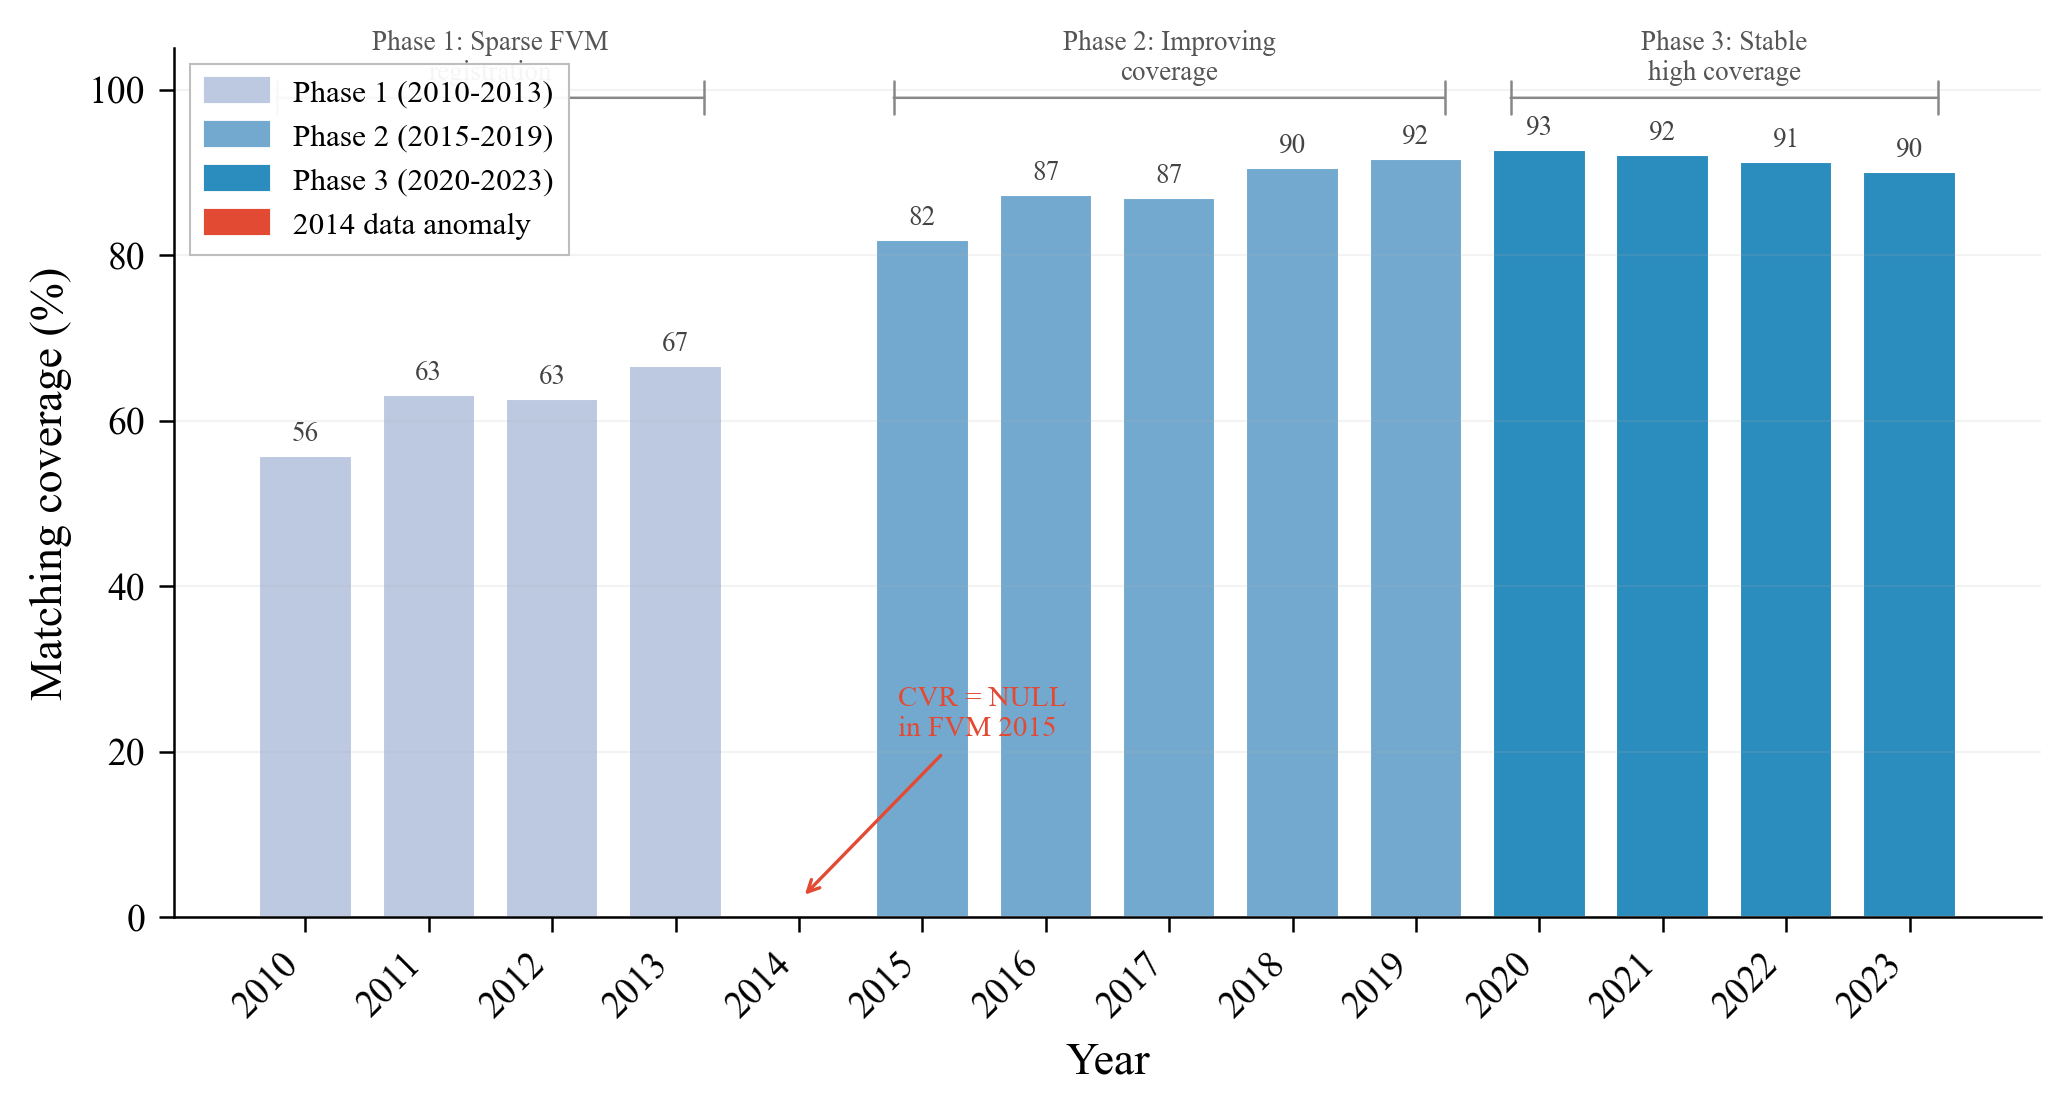
\includegraphics[width=\textwidth]{./figures/figure_2_longitudinal_coverage.png}
\caption{Longitudinal disaggregation coverage (2010--2023) at 2\% area tolerance. Three phases are annotated: sparse FVM registration (2010--2013), improving coverage (2015--2019), and stable high coverage (2020--2023). The 2014 anomaly (0\% due to NULL CVR in FVM~2015) is marked.}
\label{fig:coverage}
\end{figure}

Three phases emerge. \textbf{Phase~1 (2010--2013):} 56--67\% coverage, reflecting early-stage adoption of electronic field registration. \textbf{Phase~2 (2015--2019):} coverage rises from 82\% to 92\%, corresponding to increasingly stringent CAP requirements for digital field registration. \textbf{Phase~3 (2020--2023):} stable plateau at 90--93\%, representing the practical ceiling of deterministic area matching. The improvement reflects FVM data completeness, not algorithmic refinement---the same algorithm was applied uniformly across all years. Across the full period (excluding 2014), approximately 3.88~million of 4.85~million SJI records were matched.

\subsection{The 2014 anomaly}

Year 2014 produced 0\% coverage. Under the Y+1 alignment, SJI~2014 matches against FVM~2015, which contains 741,882 records with plausible field counts but NULL CVR values for all records. The crop code scheme is compatible; the failure is entirely attributable to missing company identifiers in the upstream dataset. We investigated whether cross-year journal number matching could recover CVR values: of 17,259 shared numeric identifiers between FVM~2016 and FVM~2017, zero had matching CVR numbers, confirming that journal numbers are year-specific application identifiers unsuitable for cross-year CVR recovery.

\subsection{Tolerance sensitivity}
\label{sec:tolerance}

Table~\ref{tab:tolerance} presents coverage across seven tolerance levels for years with consistent FVM quality (2015--2023).

\begin{table}[H]
\centering
\caption{Combined (S1+S2) coverage (\%) at seven area tolerance levels.}
\label{tab:tolerance}
\begin{tabular}{@{}lccccc@{}}
\toprule
Tolerance & 2015 & 2018 & 2020 & 2021 & 2023 \\
\midrule
0.0\% & 43.7 & 47.7 & 45.2 & 42.0 & 37.8 \\
0.5\% & 72.0 & 84.6 & 86.7 & 85.5 & 78.2 \\
1.0\% & 77.5 & 88.3 & 90.8 & 89.9 & 85.5 \\
2.0\% & 81.8 & 90.5 & 92.7 & 92.1 & 90.0 \\
3.0\% & 83.7 & 91.5 & 93.5 & 92.9 & 91.8 \\
5.0\% & 85.5 & 92.5 & 94.4 & 93.8 & 93.3 \\
10.0\% & 87.4 & 93.8 & 95.4 & 94.8 & 94.8 \\
\bottomrule
\end{tabular}
\end{table}

\begin{figure}[H]
\centering
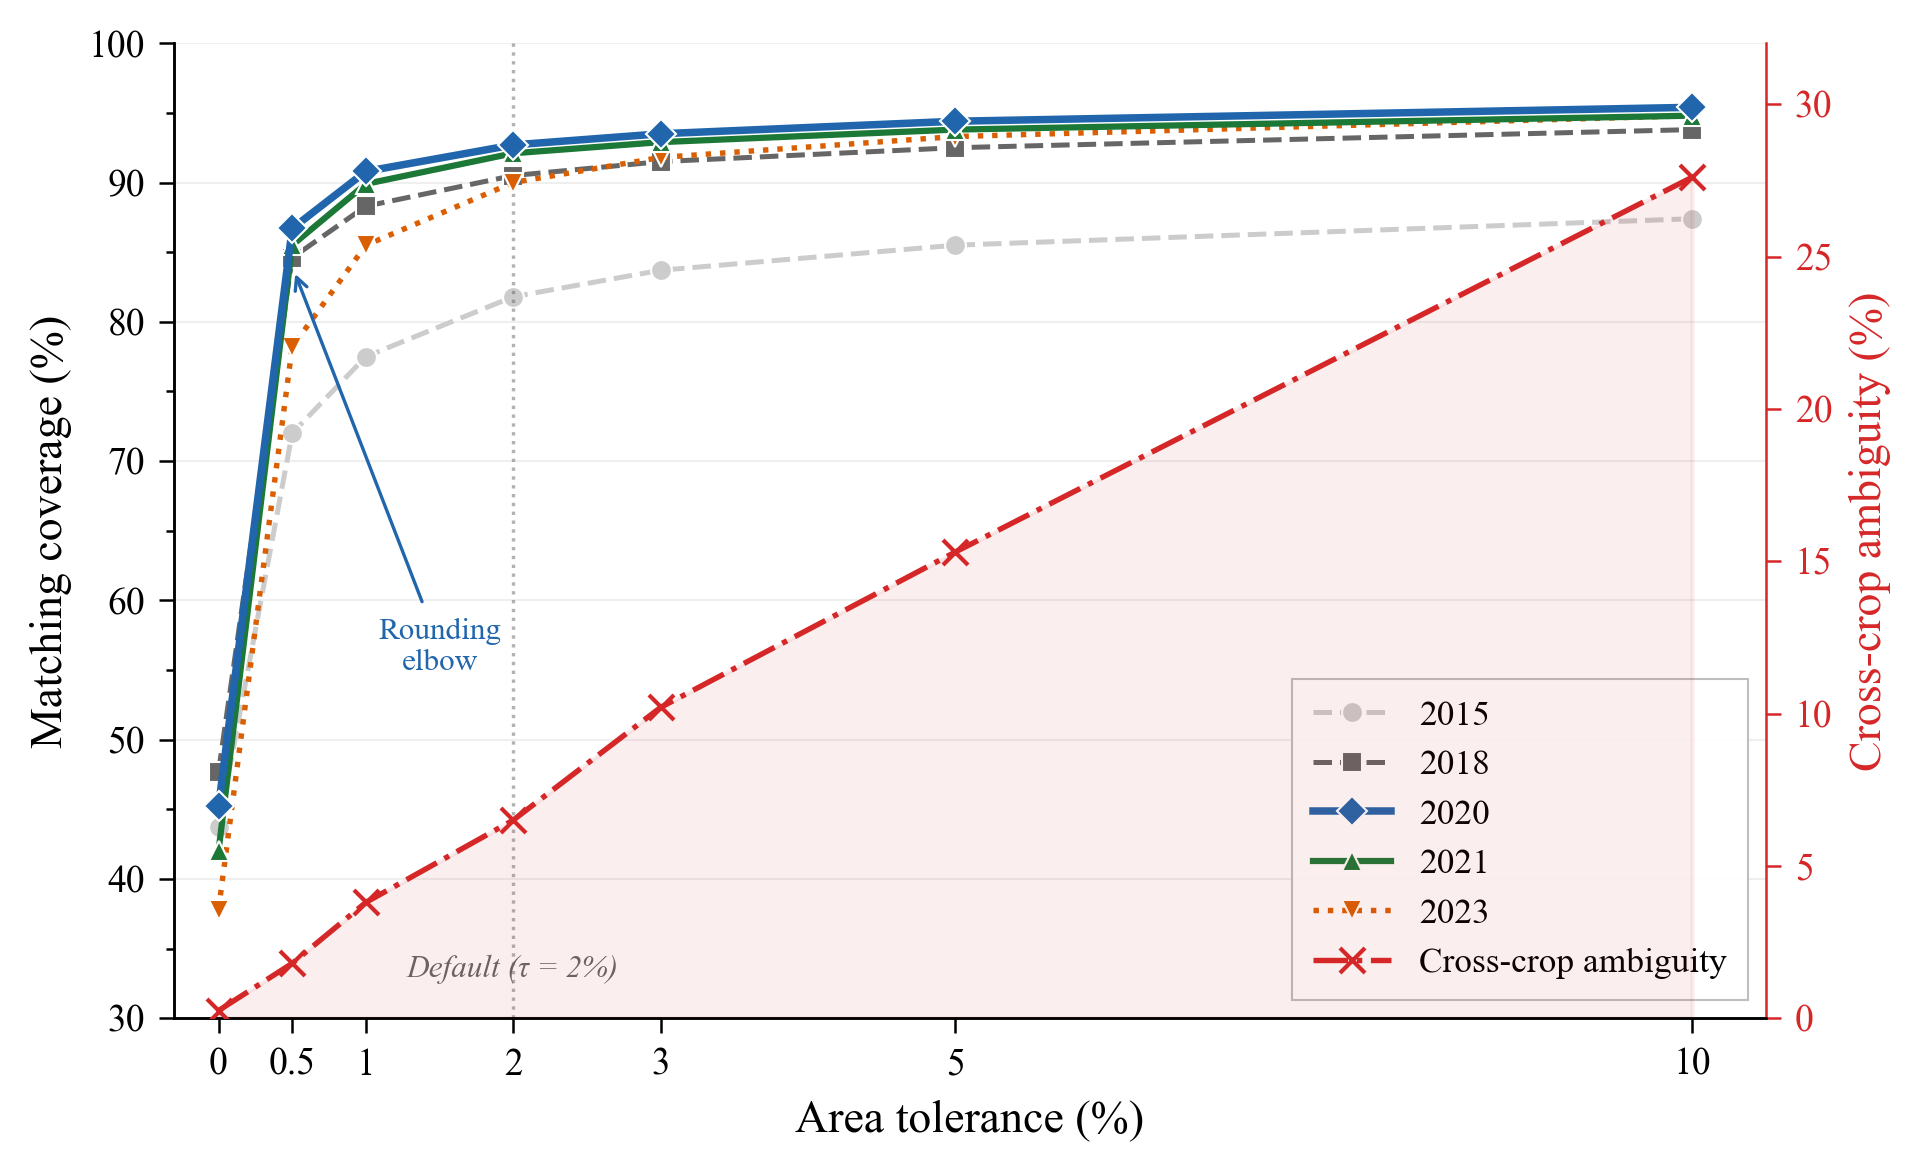
\includegraphics[width=\textwidth]{./figures/figure_1_tolerance_sensitivity.png}
\caption{Tolerance sensitivity: matching coverage versus area tolerance for selected years, with cross-crop-code ambiguity rate (right axis, 2021). The sharp elbow between 0\% and 0.5\% identifies area rounding as the dominant mismatch source. The 2\% default balances coverage against rising ambiguity.}
\label{fig:tolerance}
\end{figure}

\textbf{Area rounding is the dominant mismatch source.} The 0\% to 0.5\% jump produces the largest coverage gain in every year---from 28\,pp (2015) to 42\,pp (2020)---consistent with systematic rounding of reported areas to the nearest 0.1 or 0.5~hectare.

\textbf{Diminishing returns above 2\%.} Moving from 2\% to 10\% adds only 3--5\,pp of coverage while the cross-crop-code ambiguity rate (records matching multiple crop groups under the same CVR) rises from 6.5\% at 2\% to 27.6\% at 10\% (2021). The 2\% default represents the inflection point where coverage gains flatten and ambiguity costs accelerate.

\subsection{Allocation plausibility}

The coverage figures above measure matching success, not allocation accuracy. No independent ground-truth dataset of field-level pesticide applications exists in Denmark. The distinction between coverage and accuracy is critical.

\paragraph{Field-count distribution.} For 2021 (314,740 S1-matched records at 2\%): 19.6\% are single-field matches (unambiguous allocation), 31.9\% match 2--3 fields, 17.9\% match 4--5 fields, 18.7\% match 6--10 fields, and 11.9\% match 11+ fields. The median allocation set contains three fields. Only the 19.6\% single-field matches receive allocations free of the uniform-intensity assumption; the remaining 80.4\% are distributed proportionally by area.

\paragraph{Cross-crop ambiguity.} At 2\% tolerance, 6.5\% of matched records (20,647 of 315,114) could match multiple crop groups, rising to 27.6\% at 10\%.

\paragraph{Dose-rate plausibility.} Of 1,671,295 checkable disaggregated records (2021), 289 (0.017\%) exceeded 10 times the product-specific median dose rate (L/ha). The distribution has a mean of 0.42~L/ha and median of 0.22~L/ha. This low outlier rate suggests disaggregation does not systematically produce implausible allocations, though it cannot detect errors within the normal dose range.

\paragraph{Unmatched characterization.} Of 27,188 unmatched records (2021): 67\% have a matching CVR+crop but area deviation exceeding 2\%; 24\% have a CVR entirely absent from FVM; 8\% have CVR present but no matching crop code.

\paragraph{Summary.} True allocation accuracy is bounded above by matching coverage (92.1\%) and below by the single-field unambiguous fraction (19.6\%). Narrowing this wide bound through validation against independent data sources remains important future work.

%----------------------------------------------------------------------
\section{Discussion}

\subsection{Coverage reflects data infrastructure, not algorithmic improvement}

The rising coverage from 56\% (2010) to a plateau above 90\% (2018--2023) reflects the progressive completeness of Denmark's FVM field registration, not algorithmic refinement. Phase~1 (2010--2013) corresponds to early electronic adoption; Phase~2 (2015--2019) to CAP-mandated digital registration; Phase~3 (2020--2023) to steady-state completeness. The remaining $\sim$8\% residual represents structurally unmatchable cases: farms below the 10-hectare reporting threshold, company restructurings, or area discrepancies beyond tolerance.

\subsection{Deterministic matching versus statistical downscaling}

The method's primary advantage over statistical approaches \cite{balcaen2025,deguine2023,maggi2019} is auditability: every allocation traces to a specific CVR-crop-area match with no hidden weights or learned parameters. The single tolerance parameter is transparently characterized (Section~\ref{sec:tolerance}). These properties suit regulatory applications requiring verifiability.

An important qualification: the proportional allocation step is itself a statistical assumption---it distributes doses uniformly by area, functionally similar to area-proportional downscaling applied at farm rather than regional level. The genuine distinction is that the matching step narrows the geographic scope from a postal code or region to a single farm's fields, preserving the identity linkage. For 19.6\% of records (single-field matches), the allocation is deterministic. For the remaining 80.4\%, it is an approximation whose accuracy depends on unobserved within-farm heterogeneity of application intensity. The coefficient of variation of within-farm dose intensity across fields of the same crop is unknown and likely substantial; agronomic factors including pest pressure, soil type, and microclimate all influence field-level application decisions. Future work should quantify this uncertainty through simulation with synthetic dose heterogeneity at plausible within-farm variation levels.

\subsection{Limitations}

\textit{Uniform-intensity assumption.} Proportional allocation averages over within-farm heterogeneity. Per-field doses are correct in aggregate (mass balance is preserved) but potentially inaccurate for individual fields, particularly in large operations with many fields.

\textit{Temporal boundary stability.} The Y+1 pattern assumes field boundaries registered in year~$X+1$ correspond to fields cultivated during year~$X$. Boundary changes from splits, mergers, or sales between growing season and registration introduce mismatches of unknown magnitude.

\textit{Reporting threshold.} Farms under 10~hectares are exempt from SJI reporting. These represent 25--30\% of Danish farms but only 2--4\% of cultivated area \cite{dst2023}. Their exclusion is disproportionately relevant in peri-urban areas where proximity to residential buildings is greatest.

\textit{Systematic under-reporting.} SJI consumption is consistently below sales totals, particularly for glyphosate inter-crop applications \cite{mst2023}. Disaggregated outputs represent a lower bound.

\textit{CVR consistency.} Company restructuring, mergers, or registration errors can break the CVR linkage that is foundational to the method.

\textit{2014 data gap.} The NULL CVR column in FVM~2015 leaves one year unrecoverable without re-processing upstream data.

\subsection{Transferability and future applications}

The approach is applicable to any jurisdiction with farm-identity-linked pesticide reporting, georeferenced field boundaries under the same identifier, and a shared crop classification. The Netherlands (Basisregistratie Gewaspercelen), Belgium \cite{zucchini2022}, and Switzerland \cite{moehring2020} partially meet these prerequisites. Most significantly, SAIO (EU~2022/2379) will create the data infrastructure across all EU member states, with electronic recording from 2026. The algorithm's simplicity---a single parameter, no training data---makes adaptation straightforward.

The disaggregated dataset enables downstream applications including proximity scoring near residential buildings, PFAS exposure mapping, and regulatory compliance analysis. These are implemented as preliminary capabilities within the landbruget.dk platform but require independent validation before policy-relevant conclusions can be drawn.

\subsection{Ethics and data protection}

The method links identifiable companies (CVR) to specific pesticide applications on georeferenced fields. Under Danish and EU law, CVR numbers identify registered businesses, not natural persons. GDPR Recital~14 explicitly excludes data concerning legal persons---including company name, form, and contact details---from the regulation's scope. For sole proprietorships (\textit{enkeltmandsvirksomheder}), where the CVR is linked to a natural person, the data nonetheless pertains to professional agricultural activity rather than private life, and the CJEU \textit{Schecke} proportionality framework (C-92/09) supports publication where environmental transparency objectives are at stake.

Critically, Denmark implements the Aarhus Convention through the \textit{milj\o{}oplysningsloven} (Environmental Information Act), which establishes an affirmative right of public access to environmental information with narrowly construed exceptions. Pesticide application data falls squarely within the Convention's definition of environmental information (emissions and discharges of substances into the environment). The CVR register itself is public by statute under the CVR-loven (LBK nr.\ 1052/2019). The SJI data was obtained through FOI requests (\textit{aktindsigt}), and the landbruget.dk platform publishes CVR-level application records in its public-facing interfaces, consistent with Denmark's strong tradition of environmental data transparency. California's PUR system, by comparison, excludes grower identity from public releases---a design choice reflecting different legal traditions rather than a universal standard. Any replication of this approach in other jurisdictions must consider local data protection frameworks, but the Danish legal basis for publication is robust.

%----------------------------------------------------------------------
\section{Conclusion}

This paper presented a method for matching company-level pesticide application records to individual agricultural fields using shared administrative identifiers (CVR) and crop codes, with proportional dose allocation within a 2\% area tolerance. The matching step is deterministic and auditable; the proportional allocation step relies on an unvalidated uniform-intensity assumption.

Empirical characterization across 14~years of Danish data (2010--2023) demonstrated matching coverage exceeding 90\% from 2018 onward, peaking at 92.7\% in 2020. Coverage measures matching success, not allocation accuracy: 19.6\% of matched records receive unambiguous single-field allocations, while 80.4\% are distributed across multiple fields. Tolerance sensitivity analysis confirmed that area rounding in spray journal reporting is the dominant matching failure mode: the 0\% to 0.5\% tolerance jump produces the largest coverage gain in every year.

The method's principal limitation is the approximately 8--10\% residual of records that cannot be matched within tolerance, and the unquantified uncertainty in proportional allocation for multi-field matches. Future work should quantify allocation error through simulation with synthetic within-farm dose heterogeneity, investigate temporal stability of field boundaries across consecutive years with formal Y+0/Y+1 comparison, and extend the approach to other EU member states as SAIO-mandated electronic reporting becomes operational.

%----------------------------------------------------------------------
\section*{Data Availability Statement}

Input data are Danish government administrative records. Spray journal data (SJI) was obtained through freedom of information requests (\textit{aktindsigt}) to Milj\o styrelsen and is not publicly available. Field boundary data (FVM Marker) is publicly available via geodata.fvm.dk. The BMD pesticide registry is at bmd.mst.dk. The GEUS VP4 dataset is accessible via DOI: 10.22008/FK2/IHVDXL. The pipeline and validation script are open-source.

%----------------------------------------------------------------------
\section*{AI Disclosure Statement}

This paper was drafted with assistance from Claude (Anthropic, Claude Opus~4.6). All empirical analyses, algorithm design, and validation were performed by the authors. The AI assistant was used for literature search, prose drafting, and manuscript preparation.

%----------------------------------------------------------------------
\begin{thebibliography}{99}

\bibitem{balcaen2025} Balcaen, T., Pinsard, C., Koehl, A., Pernin, C., \& Hedde, M. (2025). Pesticides application rate maps in the European Union at a 250\,m spatial resolution. \textit{Scientific Data}, 12, Article~234.

\bibitem{cadpr2024} California Department of Pesticide Regulation. (2024). \textit{Pesticide Use Reporting}. \url{https://www.cdpr.ca.gov/pesticide-use-in-california/pesticide-use-reporting/}

\bibitem{dst2023} Danmarks Statistik. (2023). \textit{Statistikbanken: Bedrifter efter areal}. \url{https://www.statistikbanken.dk/}

\bibitem{deguine2023} Deguine, O., et al. (2023). Modelling the spatialisation of pesticide sales to monitor environmental policies in France. \textit{Journal of Cleaner Production}, 414, Article~137543.

\bibitem{deguine2025} Deguine, O., et al. (2025). From parcels to people: Development of a spatially explicit risk indicator for monitoring residential pesticide exposure. \textit{Scientific Reports}, 15, Article~5678.

\bibitem{efsa2023} EFSA. (2023). Technical report on harmonized pesticide use monitoring across EU Member States. \textit{EFSA Supporting Publications}.

\bibitem{ec2020} European Commission. (2020). \textit{A Farm to Fork Strategy for a fair, healthy and environmentally-friendly food system}. COM(2020) 381 final.

\bibitem{ec2022} European Parliament \& Council. (2022). Regulation (EU) 2022/2379 on statistics on agricultural input and output. \textit{Official Journal of the European Union}, L~315, 1--72.

\bibitem{eurostat2023} Eurostat. (2023). Agri-environmental indicator---consumption of pesticides. \textit{Statistics Explained}.

\bibitem{gutsche1997} Gutsche, V., \& Rossberg, D. (1997). SYNOPS 1.1: A model to assess the environmental risk potential of active ingredients. \textit{Agriculture, Ecosystems \& Environment}, 64(2), 175--192.

\bibitem{jrc2019} Joint Research Centre. (2019). \textit{Workshop report: Estimating pesticide use from heterogeneous data sources}. European Commission JRC, Ispra.

\bibitem{kudsk2018} Kudsk, P., J\o rgensen, L.\,N., \& \O rum, J.\,E. (2018). Pesticide Load---A new Danish pesticide risk indicator. \textit{Land Use Policy}, 70, 384--393.

\bibitem{lbst2024} Landbrugsstyrelsen. (2024). \textit{FVM Marker---WFS service for agricultural field boundaries}. \url{https://geodata.fvm.dk}

\bibitem{larsen2017} Larsen, A.\,E., \& Noack, F. (2017). Identifying the landscape drivers of agricultural insecticide use leveraging evidence from 100,000 fields. \textit{PNAS}, 114(21), 5473--5478.

\bibitem{maggi2019} Maggi, F., et al. (2019). PEST-CHEMGRIDS, global gridded maps of the top 20 crop-specific pesticide application rates. \textit{Scientific Data}, 6, Article~170.

\bibitem{mst2023} Milj\o styrelsen. (2023). \textit{Bek\ae mpelsesmiddelstatistik 2022}. \url{https://mst.dk/erhverv/sikker-kemi/pesticider/statistik/}

\bibitem{mst2024} Milj\o styrelsen. (2024). Indberetning og f\o ring af spr\o jtejournal (SJI). \url{https://mst.dk/erhverv/sikker-kemi/pesticider/}

\bibitem{moehring2020} M\"ohring, N., Gaba, S., \& Finger, R. (2020). Quantity based indicators fail to identify extreme pesticide risks. \textit{Science of the Total Environment}, 741, Article~140249.

\bibitem{nuckols2007} Nuckols, J.\,R., et al. (2007). Linkage of the California Pesticide Use Reporting Database with spatial land use data. \textit{Environmental Health Perspectives}, 115(5), 684--689.

\bibitem{piera2023} Piera, A., et al. (2023). Emissions of pesticides in the European Union: A new regional-level dataset. \textit{Scientific Data}, 10, Article~862.

\bibitem{strassemeyer2017} Strassemeyer, J., Gutsche, V., \& Ahrends, H. (2017). SYNOPS-WEB, an online tool for environmental risk assessment. \textit{Crop Protection}, 97, 28--44.

\bibitem{thorling2022} Thorling, L., et al. (2022). National assessment of long-term groundwater response to pesticide regulation. \textit{Environmental Science \& Technology}, 56(17), 12445--12455.

\bibitem{zucchini2022} Zucchini, E., et al. (2022). Mapping agricultural use of pesticides to enable research and environmental health actions in Belgium. \textit{Environmental Pollution}, 315, Article~120322.

\bibitem{zucchini2024} Zucchini, E., et al. (2024). Quantifying residents' exposure to agricultural pesticides using new geospatial approaches. \textit{Heliyon}, 10(3), Article~e25234.

\end{thebibliography}

\end{document}
